\section*{Problems}

\begin{enumerate}
\item Two blocks of different sizes and masses float in a tray of water. Each
  block is half submerged, as shown below. Water has a density of
  \SI{1000}{\kilo\gram\per\metre\cubed}. What can be concluded about the
  densities of the two blocks?
  \begin{center}
    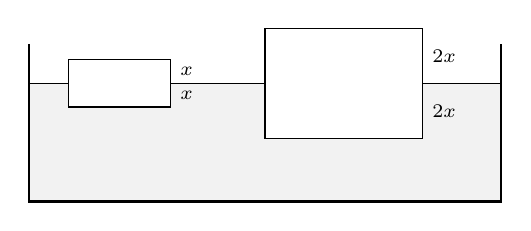
\begin{tikzpicture}
      \draw[fill=gray!10] rectangle (6,1.5);
      \draw[thick] (0,2)--(0,0)--(6,0)--(6,2);
      \draw[fill=white] (.5,1.2) rectangle (1.8,1.8);
      \draw[fill=white] (3,.8) rectangle (5,2.2);
      \node[right] at (1.8,1.65){\scriptsize $x$};
      \node[right] at (1.8,1.35){\scriptsize $x$};
      \node[right] at (5,1.85){\scriptsize $2x$};
      \node[right] at (5,1.15){\scriptsize $2x$};
    \end{tikzpicture}
  \end{center}
  \begin{enumerate}
  \item The two blocks have different densities, both of which are less than
    \SI{1000}{\kilo\gram\per\metre\cubed}.
  \item The two blocks have the same density of
    \SI{500}{\kilo\gram\per\metre\cubed}.
  \item The two blocks have the same density, but the density cannot be
    determined with the information given.
  \item The larger block has a greater density than the smaller block, but the
    densities of the blocks cannot be determined with the information given.
  \end{enumerate}
  
%  \uplevel{
%    \begin{instructions}
%      The answer to Question 1 is important in other questions in hydrostatics.
%      Once you have the answer, you can relate the proportion of mass that is
%      submerged to its density.
%    \end{instructions}
%  }

\item The figure shows four cylinders of various diameters filled to different
  heights with water. A hole in the side of each cylinder is plugged by a cork.
  All cylinders are open to the atmosphere at the top. The corks are removed.
  Which of the following is the correct ranking of the velocity of the water
  ($v$) as it exits each cylinder?
  %\cpic{.5}{mc-q2}
  \begin{enumerate}
  \item $v_A > v_D > v_C > v_B$
  \item $v_A = v_D > v_C > v_B$
  \item $v_B > v_C > v_A = v_D$
  \item $v_C > v_A = v_B = v_D$
  \end{enumerate}
  
\item A \SI1{\centi\metre} diameter pipe leads to a showerhead with twenty
  \SI1{\milli\metre} diameter exit holes. The velocity of the water in the pipe
  is $v$. What is the velocity of the water exiting the holes?
  \begin{enumerate}
  \item $0.05v$
  \item $0.5v$
  \item $5v$
  \item $100v$
  \end{enumerate}
    
  \textbf{Questions \ref{cyl1}--\ref{cyl2}}:
  Four differently shaped sealed containers are completely filled with
  alcohol, as shown below. Containers $A$ and $B$ are cylindrical.
  Containers $C$ and $D$ are truncated conical shapes. The top and bottom
  diameters of the containers are shown.
  %\cpic{.5}{mc-q3-4}
  
\item Which of the following is the correct ranking of the pressure ($P$) at
  the bottom of the containers?
  \label{cyl1}
  \begin{enumerate}
  \item $P_A = P_B = P_C = P_D$
  \item $P_A = P_D > P_C = P_B$
  \item $P_A > P_D > P_C > P_B$
  \item $P_D > P_A > P_C > P_B$
  \end{enumerate}
  
\item The force on the bottom of container $A$ due to the fluid inside
  the container is $F$. What is the force on the bottom of container $B$ due
  to the fluid inside?
  \label{cyl2}
  \begin{enumerate}
  \item $F$
  \item $F/4$
  \item $F/8$
  \item $F/16$
  \end{enumerate}
  
\item Two cylinders filled with a fluid are connected by a pipe so that fluid
  can pass between the cylinders, as shown in the figure. The cylinder on the
  right has 4 times the diameter of the cylinder on the left. Both cylinders
  are fitted with a movable piston and a platform on top. A person stands on
  the left platform. Which of the following lists the correct number of people
  that need to stand on the right platform so neither platform moves. Assume
  that the platform and piston have negligible mass and that all the people
  have the same mass.
  %\cpic{.25}{mc-q5}
  \begin{enumerate}
  \item 16 people
  \item 4 people
  \item 1 person
  \item It is impossible to balance the system because you need $1/16$ of
    a person on the right side.
  \end{enumerate}
    
\item A mass $m$ is suspended in a fluid of density $\rho$ by a string, as shown in the figure below. The tension in the string is $T$. Which of the
  following is an appropriate equation for the buoyant force $F_b$?
  \emph{Select two answers.}
  %\cpic{.25}{mc-q6}
  \begin{enumerate}
    \item$F_b=mg$
    \item$F_b=mg-T$
    \item$F_b=a^2\rho gh_1$
    \item$F_b=a^2\rho g(h_1-h_2)$
  \end{enumerate}
  
  \item Three wooden blocks of different masses and sizes float in a
  container of water, as shown in the figure. Each of the masses has a weight
  on top. Which of the following correctly ranks the buoyancy force on the
  wooden blocks?
  %\cpic{.35}{mc-q7}
  \begin{enumerate}
    \item $A > B = C$
    \item $A = B > C$
    \item $B > A = C$
    \item $B > A > C$
  \end{enumerate}
    
  %\item A beaker of water sits on a balance. A metal block with a mass of
  %\SI{70}{\gram} is held suspended in the water by a spring scale in position
  %1, as shown. In this position, the reading on the balance is
  %\SI{1260}\gram, and the spring scale reads \SI{120}\gram. When the block
  %is lifted from the water to position 2, what are the readings on the balance
  %and spring scale?
  %\cpic{.18}{mc-q10}
  %\begin{tabular}{c c c}
  %  & \underline{\textbf{Balance reading}} &
  %  \underline{\textbf{Spring scale reading}}\\
  %  (A) & \SI{1190}\gram & \SI{120}\gram \\
  %  (B) & \SI{1190}\gram & \SI{190}\gram \\
  %  (C) & \SI{1260}\gram & \SI{120}\gram \\
  %  (D) & \SI{1330}\gram & \SI{120}\gram 
  %\end{tabular}
    
%  \item Blood cells pass through an artery that has a buildup of plaque
%  along both walls, as shown in the figure. Which of the following correctly
%  describes the behavior of the blood cells as they move from the right side
%  of the figure through the area of plaque? Assume the blood cells can change
%  volume.
%  \cpic{.35}{mc-q11}
%  \begin{enumerate}
%    \item The blood cells increase in speed and expand in volume.
%    \item The blood cells increase in speed and decrease in volume.
%    \item The blood cells decrease in speed and expand in volume.
%    \item The blood cells decrease in speed and decrease in volume.
%  \end{enumerate}

   % THIS TAKEN FROM THE 2001 AP PHYSICS B EXAM FREE-RESPPONSE QUESTION #5
%  \uplevel{
%    \centering
%    \pic{.48}{submerged-block}
%    
%    \underline{Note:} Figure not drawn to scale.
%  }
%
%\item A large rectangular raft (density
%  \SI{650}{\kilo\gram\per\metre\cubed}) is floating on a lake. The surface area
%  of the top of the raft is \SI{8.2}{\metre\squared} and its volume is
%  \SI{1.80}{\metre\cubed}. The density of the lake water is
%  \SI{1000}{\kilo\gram\per\metre\cubed}.
%  \begin{parts}
%    \part Calculate the height $h$ of the portion of the raft that is above the
%    surrounding water.
%    
%    \part Calculate the magnitude of the buoyant force on the raft and state its
%    direction.
%    
%    \part If the average mass of a person is \SI{75}{\kilo\gram}, calculate the
%    maximum number of people that can be on the raft without the top of the
%    raft sinking below the surface of the water. (Assume that the people are
%    evenly distributed on the raft.)
%  \end{parts}
%  
%  % THIS IS TAKEN FROM THE 2012 AP PHYSICS B EXAM FREE-RESPPONSE QUESTION #3
%  %\uplevel{
%  %  \cpic{.3}{oils}
%  %}
%\item A glass U-tube with a uniform diameter of \SI{.850}{\centi\metre}
%  is used to determine the density of an oil. As shown in the figure above, a
%  \SI{24.5}{\centi\metre} column of water balances a \SI{27.2}{\centi\metre}
%  column of the oil so that interfaces $A$ and $B$ of the mercury with the
%  other liquids are at the same height. The density of water is
%  \SI{1.00e3}{\kilo\gram\per\metre\cubed}.
%  \begin{parts}
%    \part Calculate the density of the oil.
%    
%    \part Calculate the absolute pressure at $B$, the interface between the
%    water and the mercury.
%    
%    %\uplevel{  
%    % \cpic{.25}{u-tube}
%    A new tube, identical to the U-tube except for a cone shape on the left,
%    as shown above, is filled with the same volume of mercury that was in the
%    U-tube. The mercury is at the same height on both sides of the new tube
%    as it was in the U-tube, as shown by the dashed line. The same volumes of
%    oil and water that were in the U-tube are now poured into the new tube,
%    on the left and right respectively.
%    %}
%
%    \part Indicate the new position of $B$ relative to $A$. Justify your answer.
%    
%    \vspace{.1in}
%    \underline{\hspace{.3in}} Above $A$\hspace{.2in}
%    \underline{\hspace{.3in}} Below $A$\hspace{.2in}
%    \underline{\hspace{.3in}} At the same height as $A$
%    
%    \part A small piece of wood with density less than that of the oil is placed
%    so that it floats in the left side of the tube. Indicate whether the
%    pressure at the bottom of the tube increases, decreases, or remains the
%    same. Justify your answer.
%
%    \underline{\hspace{.3in}} Increases\hspace{.2in}
%    \underline{\hspace{.3in}} Decreases\hspace{.2in}
%    \underline{\hspace{.3in}} Remains the same
%  \end{parts}
%  
%  % THIS IS TAKEN FROM THE 2014 AP PHYSICS B EXAM FREE-RESPONSE QUESTION #2
%  \uplevel{
%    \centering
%    \begin{tikzpicture}[scale=1.3]
%      \fill[gray!50] rectangle (2,2);
%      \draw[very thick] (0,2.5)--(0,0)--(2,0)--(2,2.5);
%      \draw[very thick] (0,2)--(2,2);
%      \draw[very thick] (1,0)--(1,1);
%      \draw[very thick,fill=white] (.8,1) rectangle (1.2,1.4);
%    \end{tikzpicture}
%  }
  
%\item A cube of mass $m$ and side length $L$ is completely submerged in a
%  tank of water and is attached to the bottom of the tank by a string, as shown
%  above. The tension in the string is 0.25 times the weight of the cube. The
%  density of water is \SI{1000}{\kilo\gram\per\metre\cubed}.
%  \begin{parts}
%    %\part On the dot below that represents the cube, draw and label the forces
%    \part On the dot that represents the cube, draw and label the forces
%    (not components) that act on the cube while it is attached to the string.
%    Each force must be represented by a distinct arrow starting on, and pointing
%    away from, the dot.
%    \begin{center}
%      \vspace{.6in}
%      \tikz{\fill circle (.15);}
%      \vspace{.6in}
%    \end{center}
%    
%    \part Calculate the density of the cube.
%    
%    \part The string is now cut. Calculate the magnitude of the acceleration of
%    the cube immediately after the string is cut. If you need to draw anything
%    other than what you have shown in part (a) to assist in your solution, use
%    the space below. Do NOT add anything to the figure in part (a).
%
%    \part Indicate whether the magnitude of the buoyant force on the cube
%    increases, decreases, or remains the same while the cube is rising, but
%    before it reaches the surface.
%
%    \underline{\hspace{.3in}} Increases\hspace{.2in}
%    \underline{\hspace{.3in}} Decreases\hspace{.2in}
%    \underline{\hspace{.3in}} Remains the same
%   
%    
%    \vspace{.15in}Justify your answer.
%  \end{parts}
%
%%\uplevel{
%%  \cpic{.36}{fr-q2}
%%}
%
%tem A \SI{1.0}{\centi\metre} radius hose with a \SI{.50}{\centi\metre}
%radius exit nozzle is being used to fill a \SI1{\litre} beaker with oil
%(\SI1\litre=\SI{.001}{\metre\cubed}). The velocity of
%the oil in the hose is $v=\SI{.40}{\metre\per\second}$ as shown in the
%figure. The density of the oil is \SI{960}{\kilo\gram\per\metre\cubed}, and
%the atmospheric pressure is \SI{1.01e5}\pascal.
%
%\begin{parts}
%  \part The nozzle attached to the end of the hose has a smaller radius than
%  the hose. If the nozzle is removed from the hose, will the beaker be filled
%  faster? Justify your answer with conservation laws.
%  
%  \part Calculate the exit velocity of the oil from the nozzle.
%  
%  \part How long will it take to fill the beaker?
%  
%  \part Point A is shown in the figure. How does the pressure in the fluid at
%  point A compare to the pressure in the fluid at the exit nozzle? Justify
%  your claim.
%
%  \part The hose is now used to fill a \SI{200}{\milli\litre} graduated
%  cylinder with oil to the same height as the height of the oil in the
%  \SI{1000}{\milli\litre} beaker. Compare the net force from the oil on the
%  bottom of the \SI{200}{\milli\litre} cylinder and the
%  \SI{1000}{\milli\litre}. Explain your answer.
%  \vspace{\stretch2}
%\end{parts}
%\newpage
%
%\uplevel{
%  \centering
%  \pic{.2}{tank-x}\\
%  \underline{Note:} Figure not drawn to scale.
%
%  Figure 1
%}
%\item Tank X is a large cylindrical tank that is partially filled with
%water, as shown in Figure 1. The bottom of Tank X is connected to a short
%horizontal pipe. A valve that is initially closed can be opened to allow
%water to flow through the pipe and exit through the other end of the pipe.
%\begin{parts}
%  \part Two blocks, A and B, have identical dimensions and are placed in the
%  tank. Both blocks float at rest and are partially submerged in the water.
%  \begin{subparts}
%    \subpart The water and air can be modeled as consisting of individual
%    particles that are in continuous random motion. In terms of interactions
%    with both water and air particles, explain why there is an upward buoyant
%    force exerted on each block.
%    \vspace{\stretch1}
%    
%    \subpart The valve is then opened, and water flows out through the pipe.
%    The surface of the water moves downward. When Block A touches the bottom
%    of Tank X, Block B is still above the bottom of Tank X. Which block has
%    a greater density? Briefly explain your reasoning.
%    \vspace{\stretch1}
%  \end{subparts}
%  \newpage
%  
%  \uplevel{
%    \begin{center}
%      \pic{.14}{tank-y}\\
%      \underline{Note:} Figure not drawn to scale.
%
%      Figure 2
%    \end{center}
%    Tank Y is a large tank with the top open to the air, as shown in Figure
%    2. The bottom of Tank Y is connected to a short horizontal pipe of radius
%    $r$ with a closed valve. Tank Y is filled with water to height $h_0$
%    above the horizontal pipe. Tank Y is specially designed so that when the
%    valve is opened, the surface of the water moves downward at constant
%    speed $v_s$.
%  }
%  \part At time $t=0$, the valve is opened.
%  \begin{subparts}
%    \subpart Derive the relationship between the speed $v_p$ at which water
%    exits the pipe and the changing height $h$ of the surface of the water
%    above the pipe to show that $v_p = \sqrt{v_s^2 + 2gh}$.
%    \vspace{\stretch1}
%    
%    \subpart Derive the relationship between $v_p$ and the changing radius $R$
%    of the top surface of the water to show that $v_p =\dfrac{R^2}{r^2}v_s$.
%    \vspace{\stretch1}
%    
%    \subpart When the radius $R$ of the tank is sufficiently greater than
%    $r$, the speed $v_p$ can be approximated as $v_p =\sqrt{2gh}$. Justify
%    this claim.
%    \vspace{\stretch1}
%  \end{subparts}
%  \newpage
%
%  \uplevel{
%    \begin{center}
%      \pic{.17}{tank-z}\\
%      \underline{Note:} Figure not drawn to scale.
%      
%      Figure 3
%    \end{center}
%    Tank Z is a large tank whose top is open to the air and is shaped as
%    shown in Figure 3. The bottom of Tank Z is connected to a short
%    horizontal pipe with a closed valve. Tank Z is filled with water to a
%    height $h_0$ above the horizontal pipe.
%    
%    \vspace{.15in}At time $t=0$, the valve of Tank Z is opened.
%  }
%  \part Does the speed $v_s$ at which the surface of the water moves downward
%  increase, decrease, or remain the same over time as water exits the other
%  end of the pipe? Justify your answer by using or referencing equations from
%  both part (b)(i) and part (b)(ii).
%\end{parts}
%
% \item A large pan is filled to the top with oil of density $\rho_o$. A
% plastic cup of mass $m_C$, containing a sample of known mass $m_S$, is placed
% in the oil so that the cup and sample float, as shown above. The oil that
% overflows from the pan is collected, and its volume is measured. The
% procedure is repeated with a variety of samples of different mass, and the
% pan is refilled each time.
% \begin{parts}
%   \part On the dot below that represents the cup-sample system, draw and
%   label the forces (not components) that act on the system when it is
%   floating on the surface of the oil.
%
%   \vspace{.3in}
%   \begin{center}
%     {\tikz\fill circle (.2);}
%   \end{center}
%   \vspace{.3in}
%   
%   \part Derive an expression for the overflow volume $V_O$ (the volume of oil
%   that overflows due to the floating system) in terms of $\rho_0$, $m_S$,
%   $m_C$, and fundamental constants. If you need to draw anything other than
%   what you have shown in part (a) to assist in your solution, use the space
%   below. Do NOT add anything to the figure in part (a).
%
%   \uplevel{
%     Assume that the following data are obtained for the overflow volume
%     $V_O$ for several sample masses $m_S$.
%     \begin{center}
%       \begin{tabular}{|l|c|c|c|c|c|c|}
%         \hline
%         Sample mass $m_S$ (kg)
%         & 0.020
%         & 0.030
%         & 0.040
%         & 0.050
%         & 0.060
%         & 0.070\\ \hline
%         Overflow volume $V_O$ (\si{\metre\cubed})
%         & \num{29e-6}
%         & \num{38e-6}
%         & \num{54e-6}
%         & \num{62e-6}
%         & \num{76e-6}
%         & \num{84e-6}\\
%         \hline
%       \end{tabular}
%     \end{center}
%   }
%   \newpage
%   
%   \part Graph the data on the axes below, plotting the overflow volume as a
%   function of sample mass. Place numbers and units on both axes. Draw a
%   straight line that best represents the data.
%   
%   \begin{tikzpicture}[scale=.8,yscale=.6]
%     \draw[very thick,->](0,0)--(17,0) node[right]{$m_S$};
%     \draw[very thick,->](0,0)--(0,19) node[pos=0,left]{$O$} node[left]{$V_0$};
%     \draw[thick,dashed](0,0) grid(16,18);
%   \end{tikzpicture}
%
%   \part Use the slope of the best-fit line to calculate the density of the
%   oil.
%   
%   \part What is the physical significance of the intercept of your line with
%   the vertical axis?
% \end{parts}
%
% \uplevel{
%   \centering
%   {\large\textbf{BONUS QUESTION--WE WILL NOT REVIEW THIS QUESTION IN CLASS}}
%   
%   \pic{.27}{fr-2a}
% }
% 
% \item A cube of lead with a side dimension of \SI{5.0}{\centi\metre} is
% slowly lowered into the beaker of water by a thin string attached to a spring
% scale at a constant rate, as shown above. The density of lead is
% \SI{11300}{\kilo\gram\per\metre\cubed} and the density of water is
% \SI{1000}{\kilo\gram\per\metre\cubed}.
% 
% \begin{parts}
%   \part What will be the spring scale reading, in newtons, when the lead has
%   been submerged to location 2?
%   \vspace{\stretch1}
%   
%   \part Does the spring scale reading increase, decrease, or stay the same
%   when the cube is lowered from location 2 to location 3? Justify your
%   answer by referencing the pressure of the fluid on the lead cube.
%   \vspace{\stretch1}
%   
%   \part The lead cube is lowered from above the water surface (location 1) to
%   a spot just below the surface (location 2) until the cube is just above
%   the bottom of the beaker (location 3). Describe any changes in pressure
%   on the bottom of the beaker during this process. Explain your answer.
%   \vspace{\stretch1}
% \end{parts}
\end{enumerate}
